\begin{table}
  \centering
  \begin{tabular}{c c c c c}
    \toprule
    $\su{Metall}$  & $\su{Ordnungszahl} \,\, \su{Z}$ &
    $E^\su{Lit}_\su{K} \,/\, \keV$ & $\theta^\su{Lit}_\su{K}\,/\,\si{degree}$ & $\sigma^\su{K}$ \\
    \midrule
     Zn & 30 & 9.65 & 18.6 &  \\
     Ge & 32 & 11.11 & 16.1 &  \\
     Br & 35 & 13.47 & 13.2 &  \\
     Sr & 38 & 16.10 & 11.0 &  \\
     Zr & 40 & 17.09 & 9.0 &  \\
     Au & 79 & 13.70 & 13.0 (LII) &  \\
     Au & 79 & 11.92 & 15.0 (LIII) &  \\
    \bottomrule
  \end{tabular}
  \caption{Literaturwerte der Metalle \cite{Elit},\,\cite{KAu}}
  \label{tab:info}
\end{table}

\begin{figure}
  \centering
  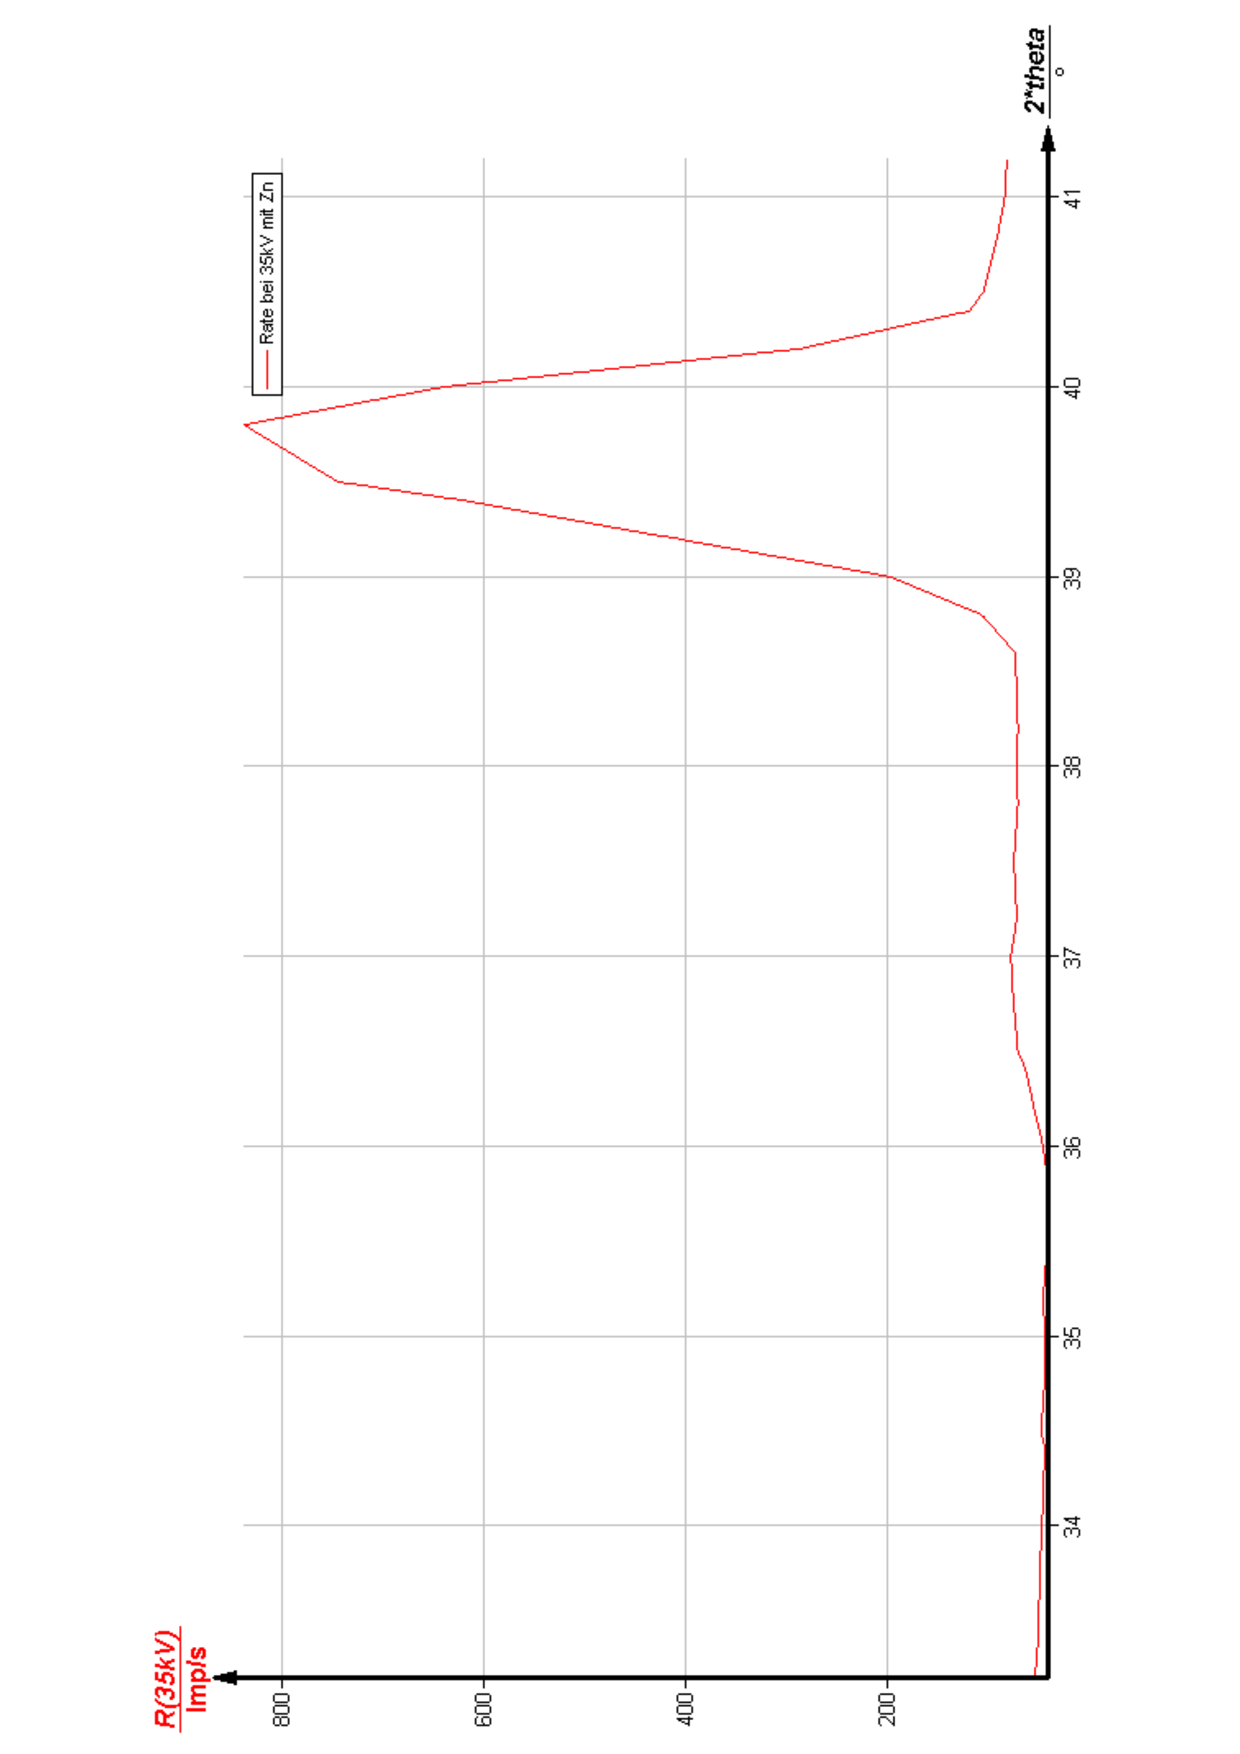
\includegraphics[width=10cm]{bilder/AbsorpZn.pdf}
  \caption{Absorptionsspektrum von Zink}
  \label{fig:Zink}
\end{figure}

\begin{figure}
  \centering
  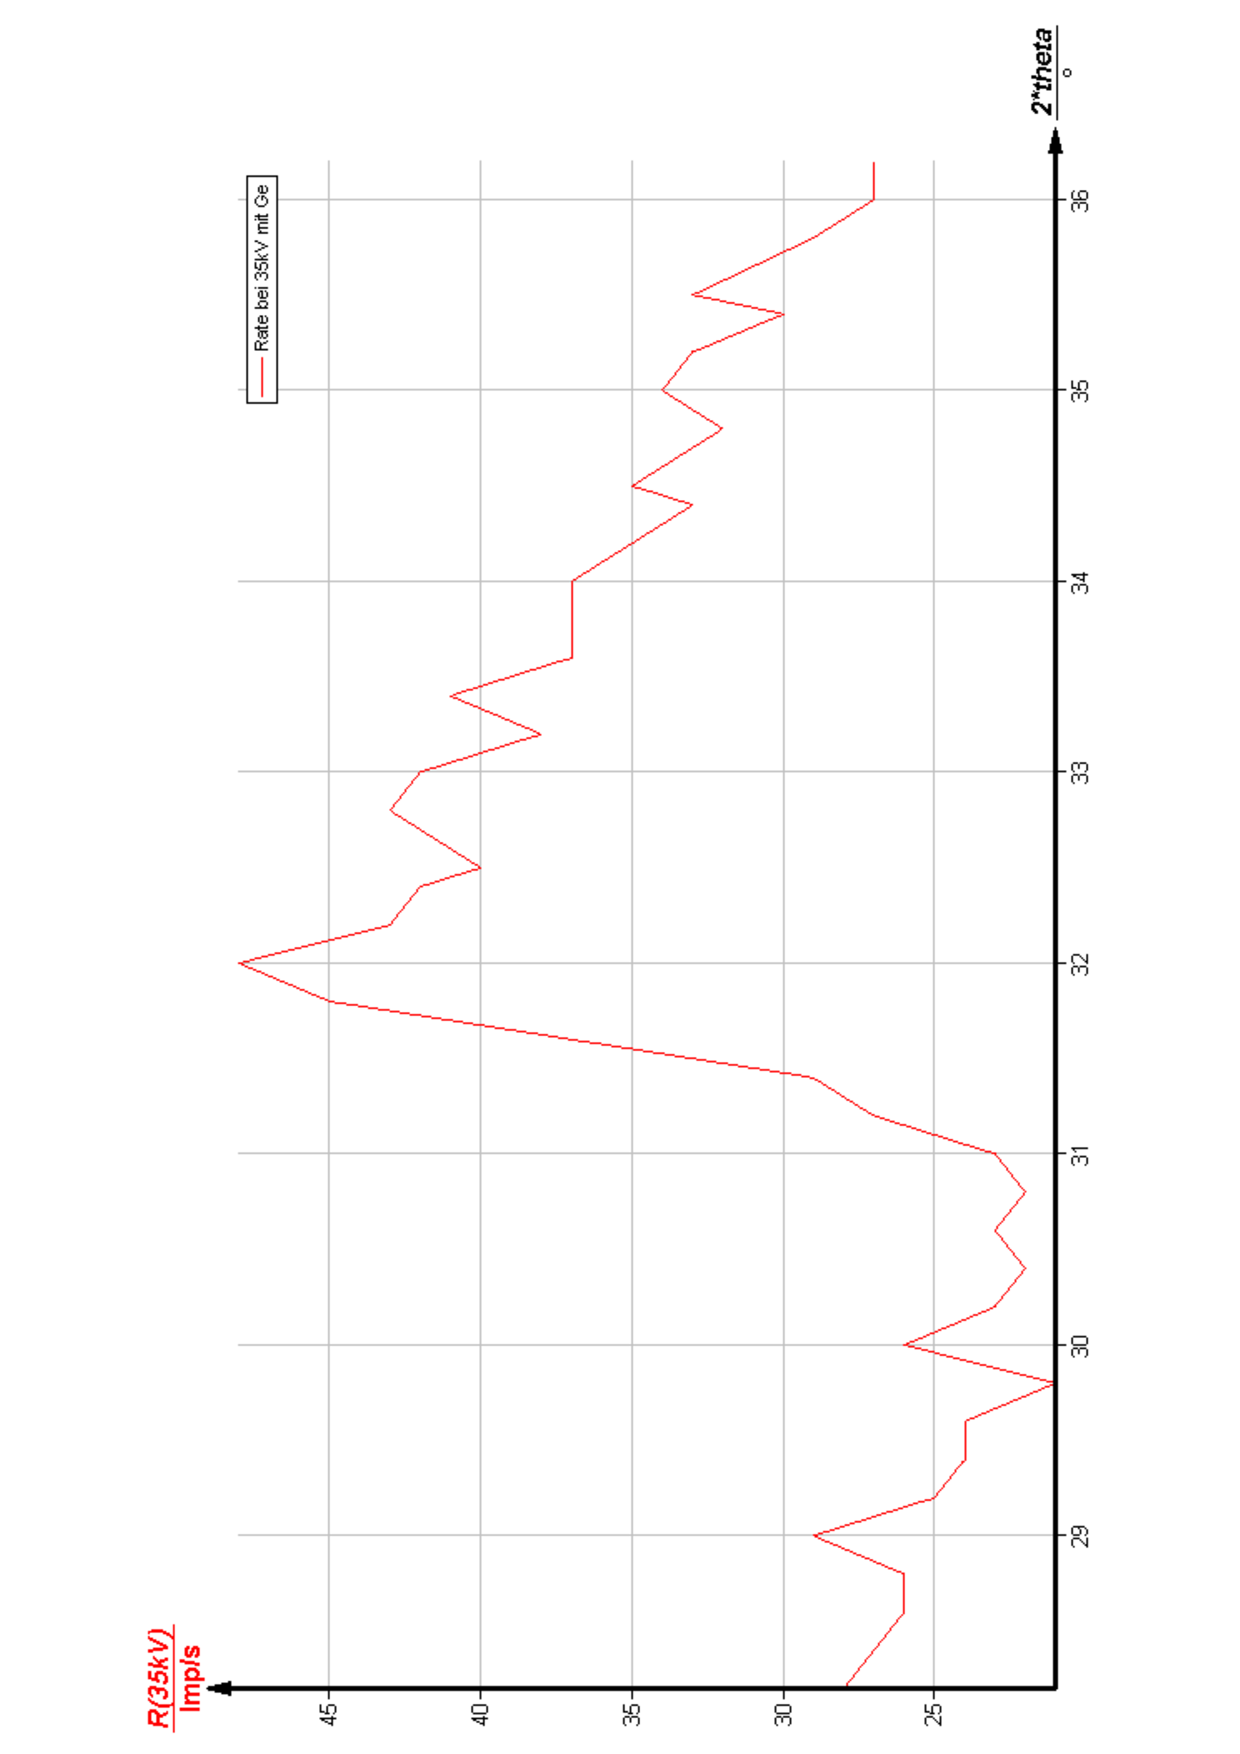
\includegraphics[width=10cm]{bilder/AbsorpGe.pdf}
  \caption{Absorptionsspektrum von Germanium}
  \label{fig:Germanium}
\end{figure}

\begin{figure}
  \centering
  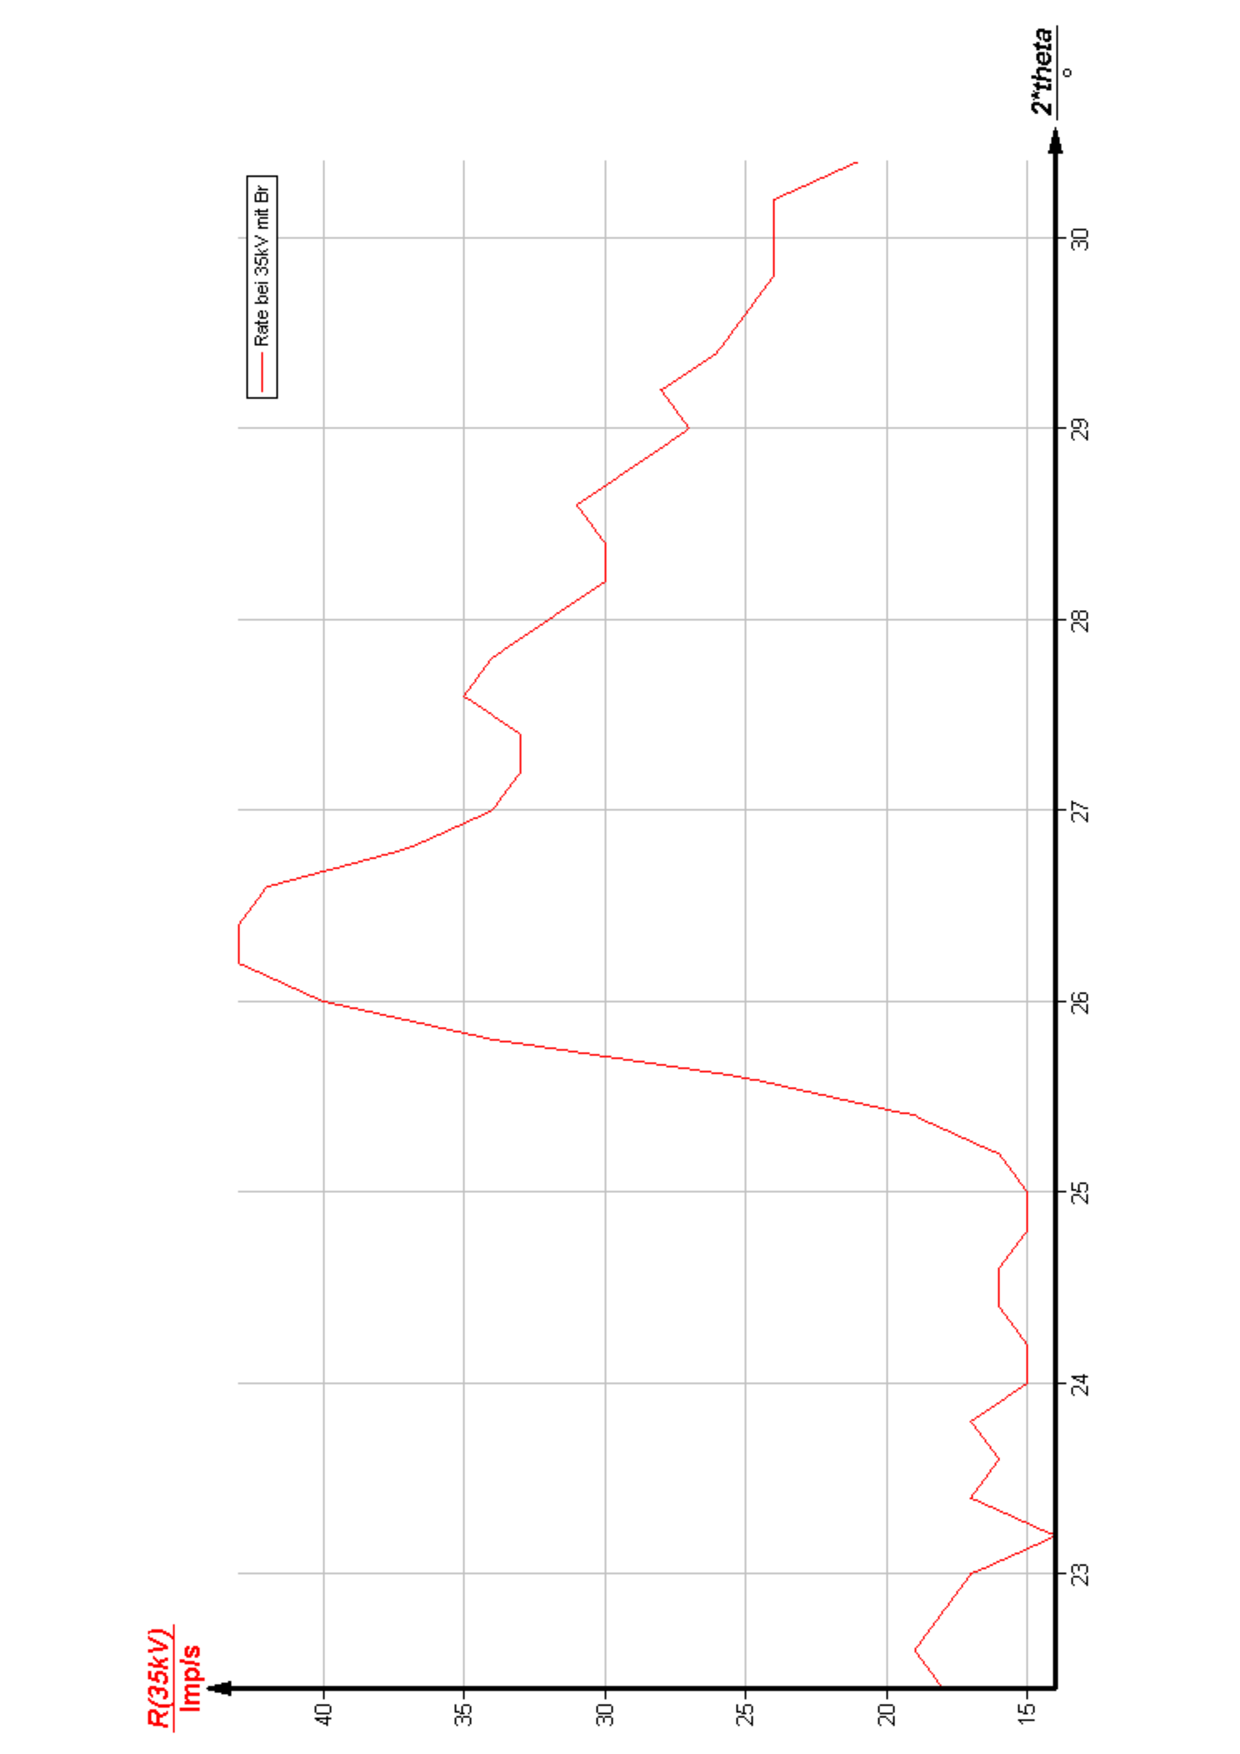
\includegraphics[width=10cm]{bilder/AbsorpBr.pdf}
  \caption{Absorptionsspektrum von Brom}
  \label{fig:Brom}
\end{figure}

\begin{figure}
  \centering
  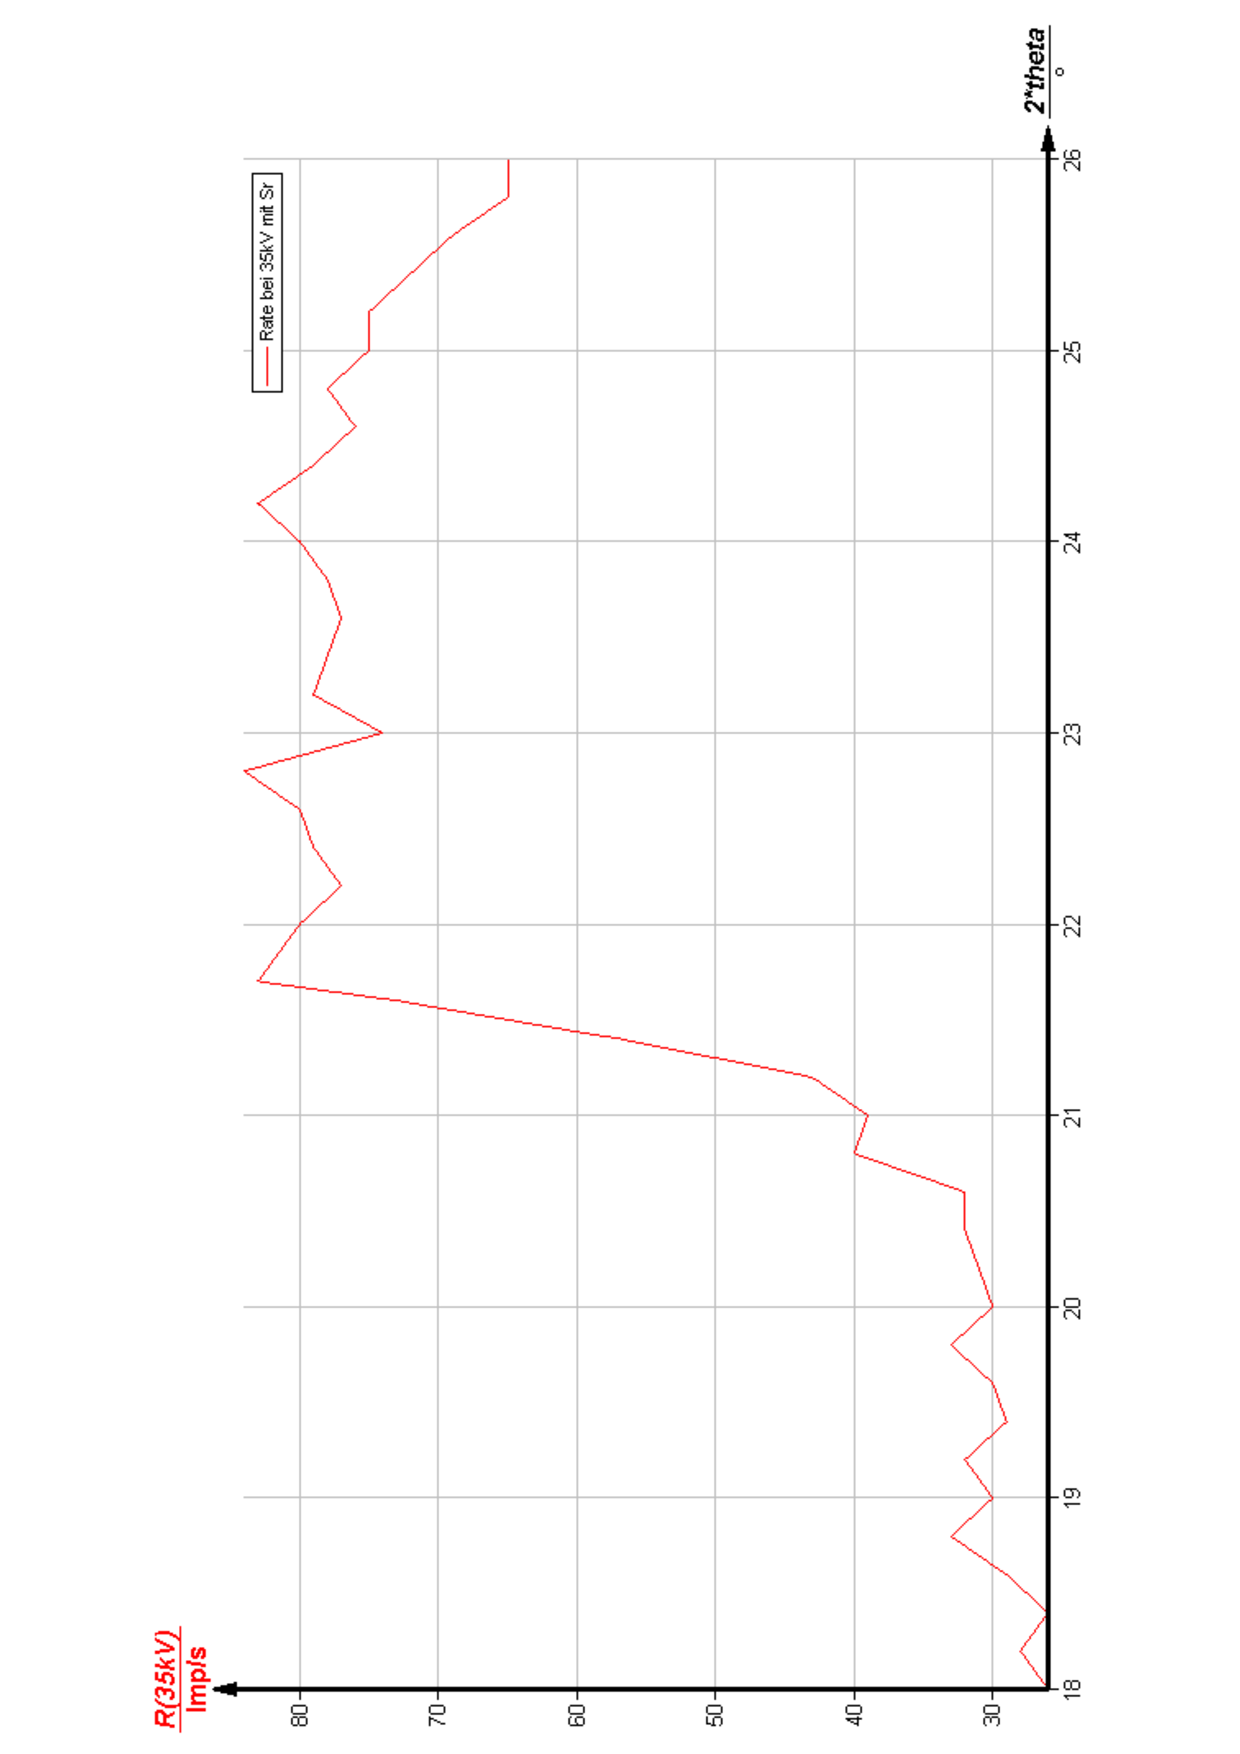
\includegraphics[width=10cm]{bilder/AbsorpSr.pdf}
  \caption{Absorptionsspektrum von Strontium}
  \label{fig:Strontium}
\end{figure}

\begin{figure}
  \centering
  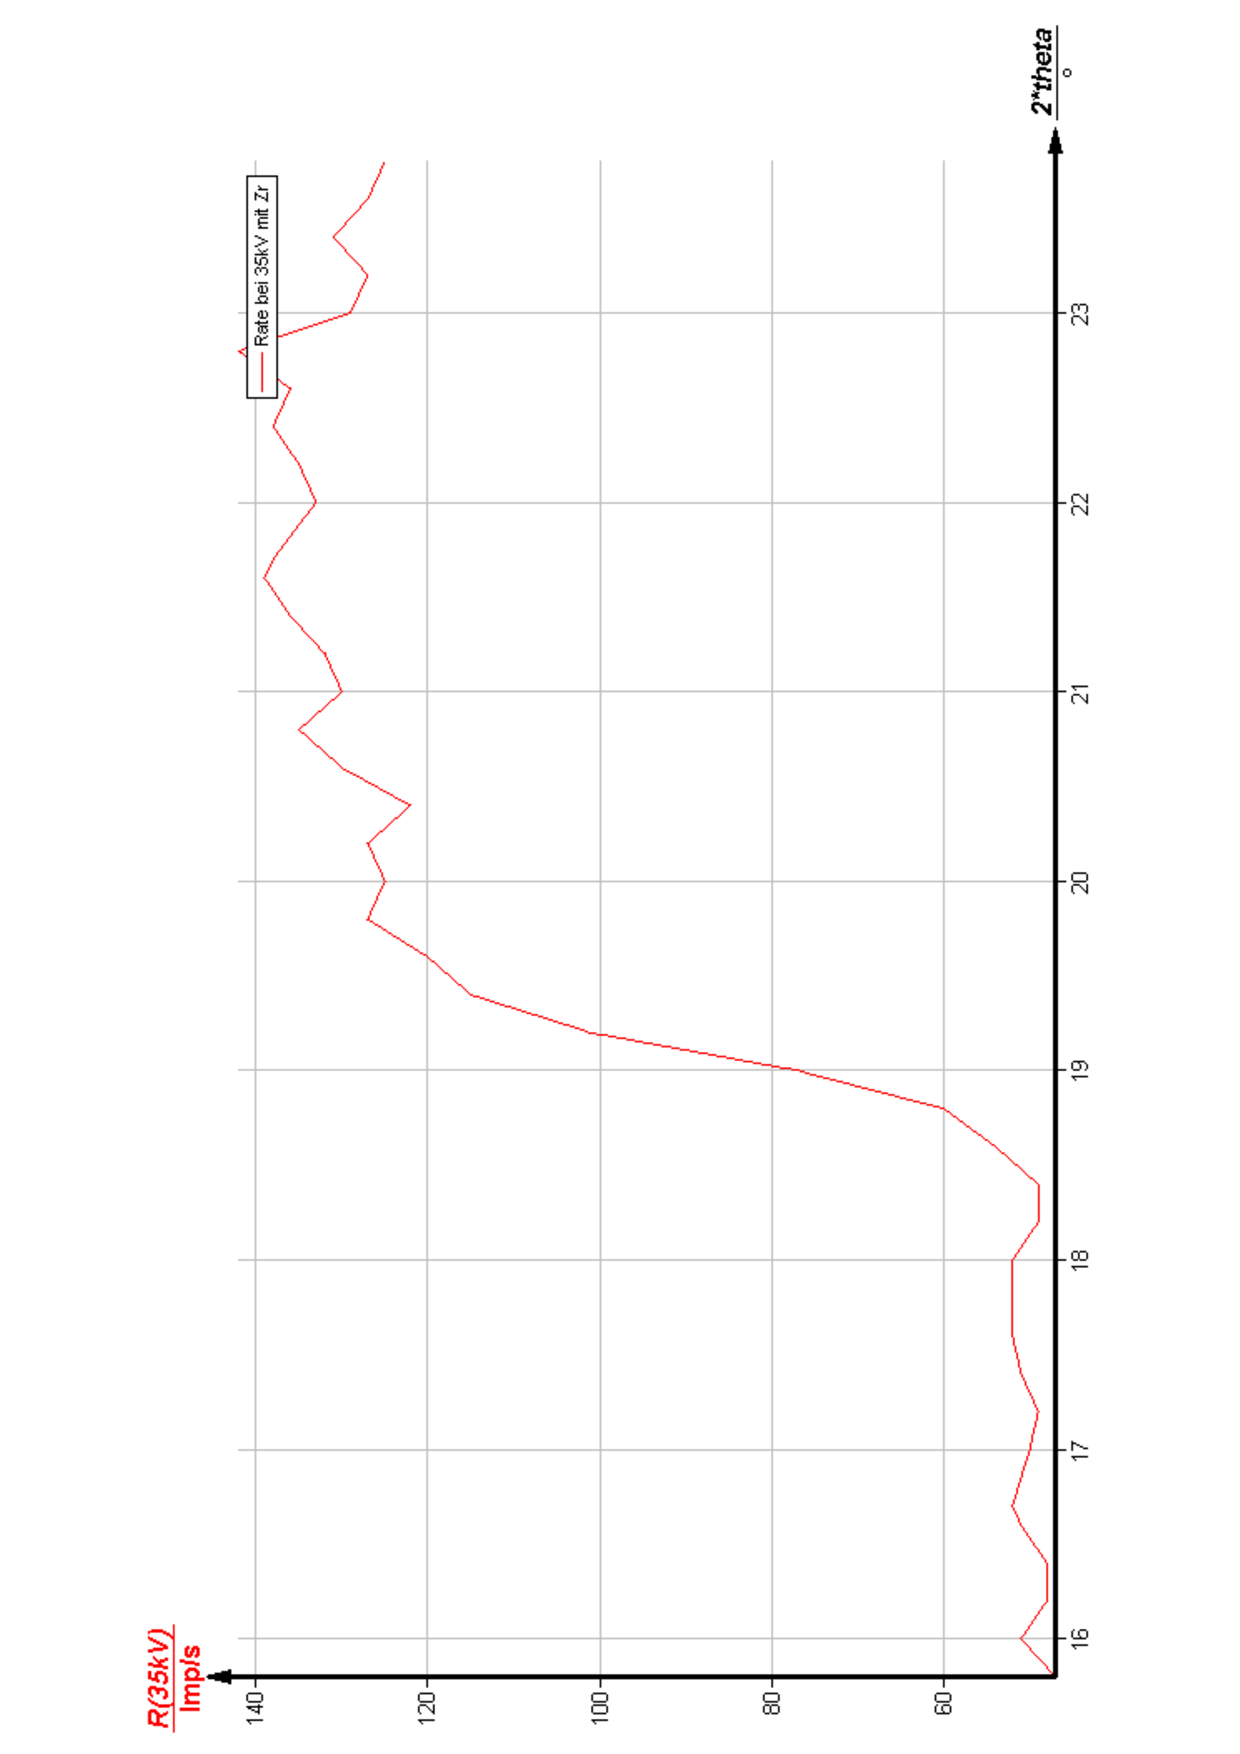
\includegraphics[width=10cm]{bilder/AbsorpZr.pdf}
  \caption{Absorptionsspektrum von Zirkonium}
  \label{fig:Zirkonium}
\end{figure}

\begin{figure}
  \centering
  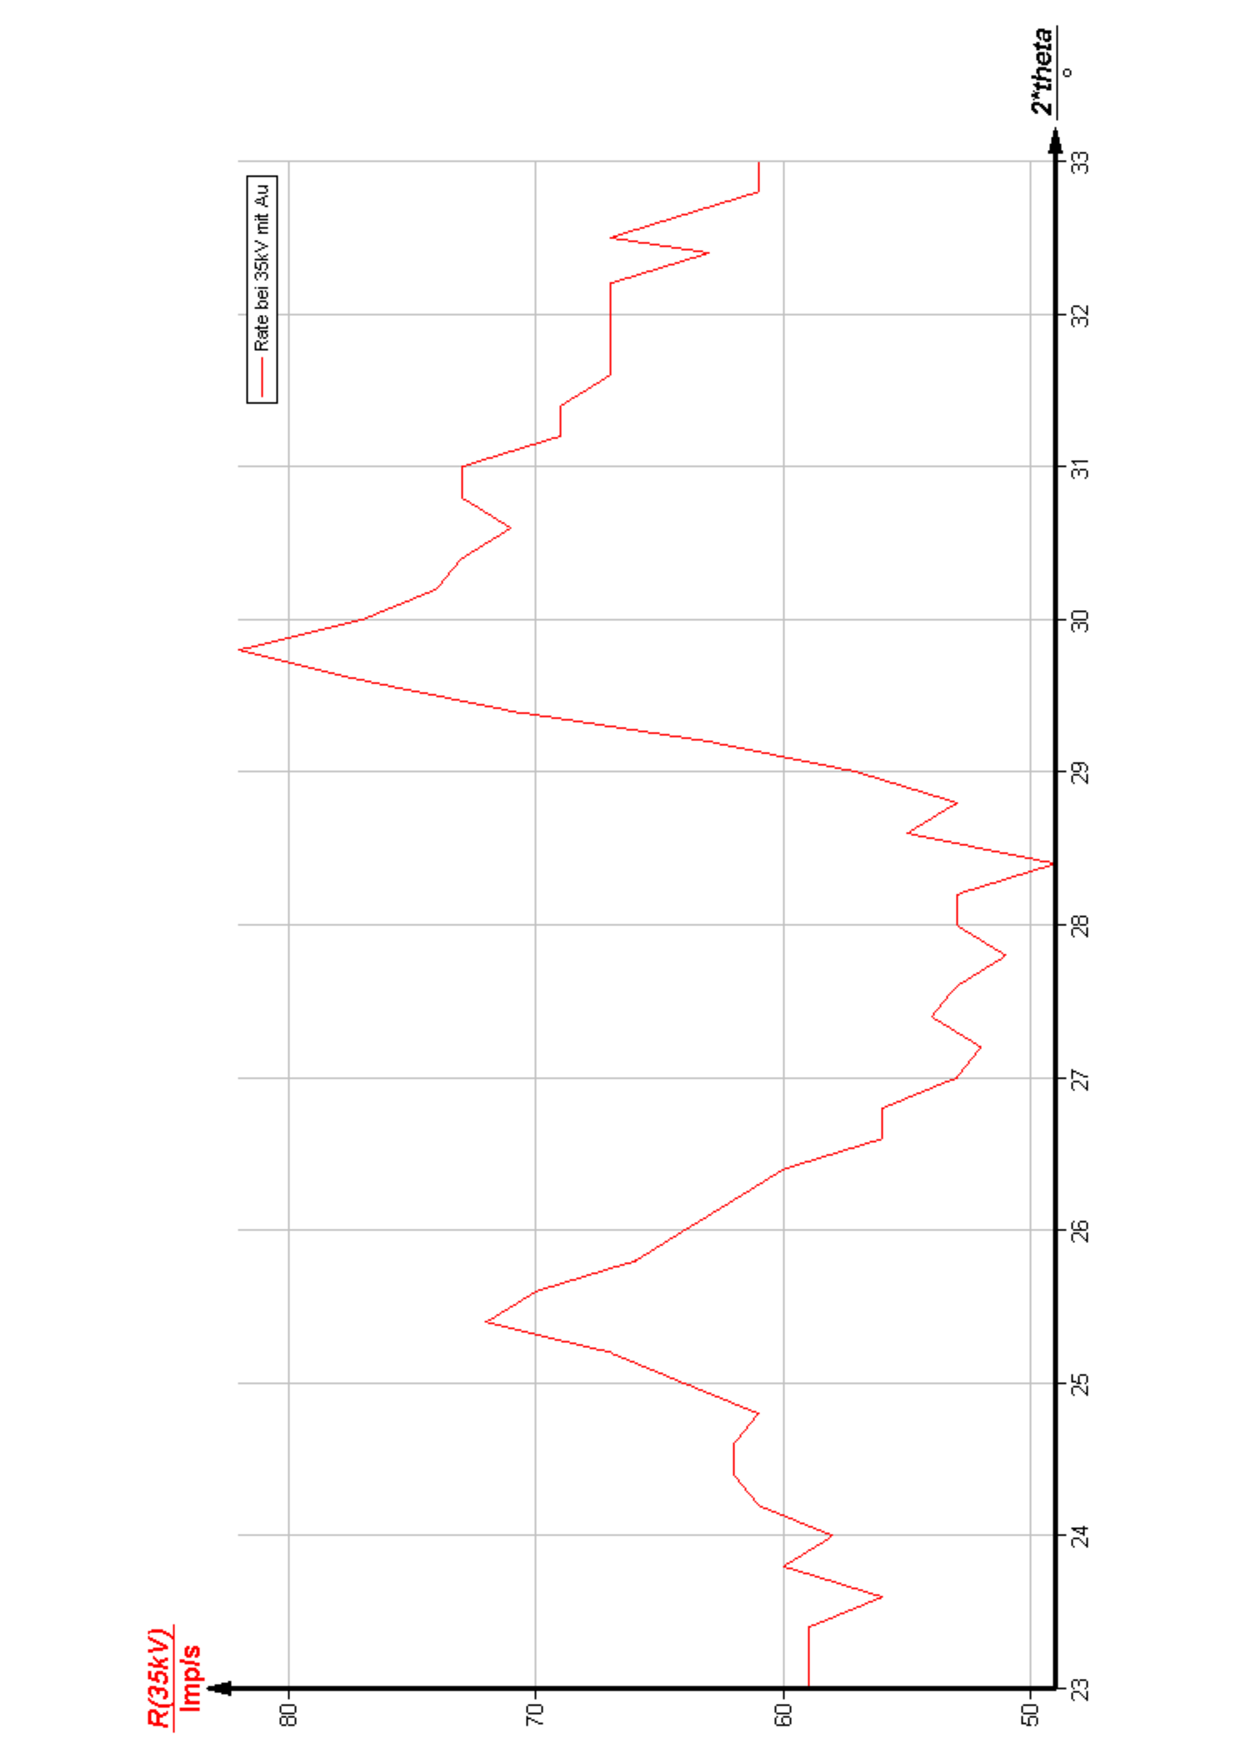
\includegraphics[width=10cm]{bilder/AbsorpAu.pdf}
  \caption{Absorptionsspektrum von Aurum}
  \label{fig:Aurum}
\end{figure}
